
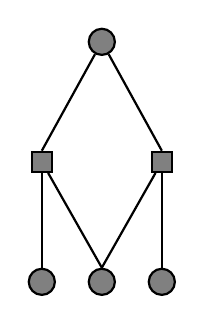
\begin{tikzpicture}
\def \depth{0.6in}; %vertical gap between nodes/levels
\def \gap{0.3in}; %Horizontal gap between nodes
\def \gapA{0.15in}; %Encoder Width
\def \textoffs{0.12in}; %Offset for writing text above a node
\def\nodewidth{0.1in};
\tikzstyle{check} = [rectangle, draw, text centered, thick, fill=gray,
                          minimum height=\nodewidth, minimum width=\nodewidth]
\tikzstyle{bit} = [circle, draw, text centered, thick, fill=gray,
                          radius=0.5*\nodewidth]
                          
\def \fsize{\normalsize}; %Defining a generic font size to be adjusted depending on the scaling
\def \dotsize{\Huge}; %Defining a generic font size to be adjusted depending on the scaling


\node [bit](b1) at (0,0) {} ;

%Level 2
\node[check] (c21) at ([xshift=-\gap,yshift=-\depth]b1) {};
\node[check] (c22) at ([xshift=+\gap,yshift=-\depth]b1) {};

%Lines form level 1-level 2
\draw[thick](b1)--(c21.north);
\draw[thick](b1)--(c22.north);

%Level 3
\node[bit] (b31) at ([xshift=0,yshift=-\depth]c21) {};
\node[bit] (b32) at ([xshift=+\gap,yshift=-\depth]c21) {};
\node[bit] (b33) at ([xshift=0,yshift=-\depth]c22) {};

%Lines form level 2-level 3
\draw[thick](c21)--(b31.north);
\draw[thick](c21)--(b32.north);
\draw[thick](c22)--(b33.north);
\draw[thick](c22)--(b32.north);

\end{tikzpicture}